\chapter{Methods and experimental setup}\label{ch:methods}
\thispagestyle{pagestyle}

\graphicspath{{../../outputs/}{images/}{../../thesis/design/figures/}}

\section{Notation and registers}
Let $N\in\{4,8,16\}$ be the linear image size. Pixels are indexed by $p\in\{0,\ldots,N^2-1\}$ with $N_{\mathrm{pix}}=N^2=2^m$ and $m=2\log_2 N$. The FRQI data register consists of one \emph{color} qubit $c$ and $m$ \emph{position} qubits ordered so that $c$ is the least significant bit in the computational basis index, matching \texttt{src/frqi.py} and \texttt{src/improved.py}. Ancillas used only for multi-controlled decomposition are denoted $a_j$ when present.

\section{Image representation and FRQI encoding}
Grayscale test images are \texttt{uint8} arrays $I[p]\in\{0,\ldots,255\}$. FRQI encodes each pixel as an $R_y$ angle on the color qubit conditioned on the address register $\ket{p}$~\cite{Le2011FRQI}. With $\theta_p = \frac{\pi}{2}\cdot\frac{I[p]}{255}$, the ideal FRQI pure state can be written schematically as
\begin{equation}
\ket{\psi_{\mathrm{FRQI}}} \propto \sum_{p=0}^{N_{\mathrm{pix}}-1} \ket{p}\otimes R_y(\theta_p)\ket{0}_c ,
\end{equation}
up to normalization conventions fixed by the implementation. The circuit prepares this state by iterating over addresses; each iteration uses multi-controlled $X$ gates to compare the position register to a binary pattern for $p$, applies $R_y(2\theta_p)$ on $c$ (Qiskit convention), then uncomputes the comparators.

\subsection{Sequential preparation routine (logical view)}
\label{sec:frqi-seq}
The address-wise pattern below matches \texttt{src/frqi.py} and \texttt{src/improved.py}; structural variants differ only in how multi-controlled $X$ layers are synthesized, not in the intended output state.
\begin{enumerate}[label=\textbf{\arabic*.}, leftmargin=*]
  \item Initialize all qubits to $\ket{0}$; apply Hadamards to the position register so $\sum_p \ket{p}$ is uniform.
  \item For each pixel address $p$, compare the position register to the binary expansion of $p$ using multi-controlled $X$ ladders, apply the controlled $y$-rotation on $c$, then uncompute comparisons to restore ancillas and the position superposition.
  \item Return the circuit; transpilation to \texttt{\{cx,rz,sx\}} occurs later at a fixed optimization level.
\end{enumerate}
This loop structure is why resource studies focus on per-pixel multi-controlled cost: it repeats $N_{\mathrm{pix}}$ times with only the rotation angle changing.

\section{QHED baseline and classical Sobel reference}
The quantum Hadamard edge detector applies a two-dimensional fast Walsh--Hadamard transform (FWHT) to the classical image reconstructed from the simulated FRQI state, forms a magnitude spectrum as a contrast proxy, inverts back to the spatial domain, and finally applies a classical $3\times 3$ Sobel magnitude filter~\cite{Yao2017QHED,QiskitTextbookQuantumEdgeDetection}. Classical Sobel on the original clean image provides the reference edge map for SSIM/PSNR comparisons. This pipeline is implemented in \texttt{src/qhed.py}.

\section{Structural FRQI preparation}
Same logical FRQI state is being realized using two Qiskit \texttt{MCXGate} modes:
\begin{itemize}
  \item \textbf{Naive (\texttt{noancilla}):} no dedicated ancillas; decomposition can incur high CX counts per multi-controlled slice~\cite{Zindorf2024EfficientMCG}.
  \item \textbf{V-chain (\texttt{v-chain}):} uses up to $m-2$ dirty ancillas to lower CX depth after transpilation~\cite{Vale2023MCSU2,Azevedo2024LowDepthMCG}.
\end{itemize}
Full naive transpilation is run for $4\times 4$. Additionally, for $8\times 8$ and $16\times 16$, it is reported \texttt{struct\_naive\_slice\_scaled} by transpiling one representative pixel slice and multiplying reported depth/CX by $N_{\mathrm{pix}}$; this is an engineering extrapolation, not a fully optimized global circuit~\cite{Arsoski2024MCXQFT}.

\subsection{Schematics: toy naive versus v-chain}
\Cref{fig:toy-naive-vchain} contrasts a three-qubit address register plus one color qubit in the naive \texttt{noancilla} view (one conceptual multi-controlled rotation block) against an ancilla-assisted v-chain slice (MCX ladder, controlled $R_y$, uncompute). The drawing is qualitative: real FRQI circuits repeat the inner pattern for every pixel address. Figures are generated by \texttt{scripts/toy\_and\_block\_level\_diagrams.py} and stored under \path{thesis/design/figures/}.

\begin{figure}[htbp]
\centering
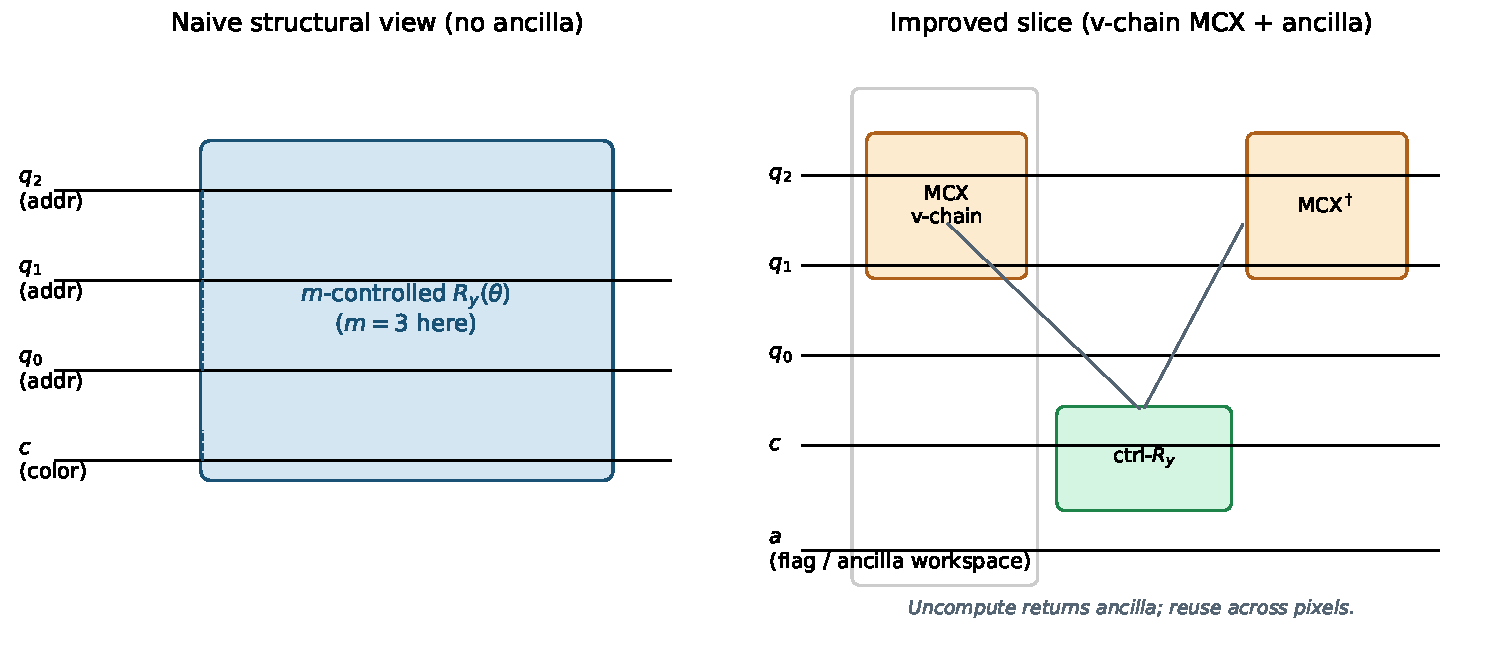
\includegraphics[width=\textwidth]{toy_naive_vs_vchain.pdf}
\caption{Toy $m{=}3$ address qubits and one color wire: naive ``all controls into one box'' versus v-chain ancilla workspace (repository figure \texttt{toy\_naive\_vs\_vchain}).}
\label{fig:toy-naive-vchain}
\end{figure}

\begin{figure}[htbp]
\centering
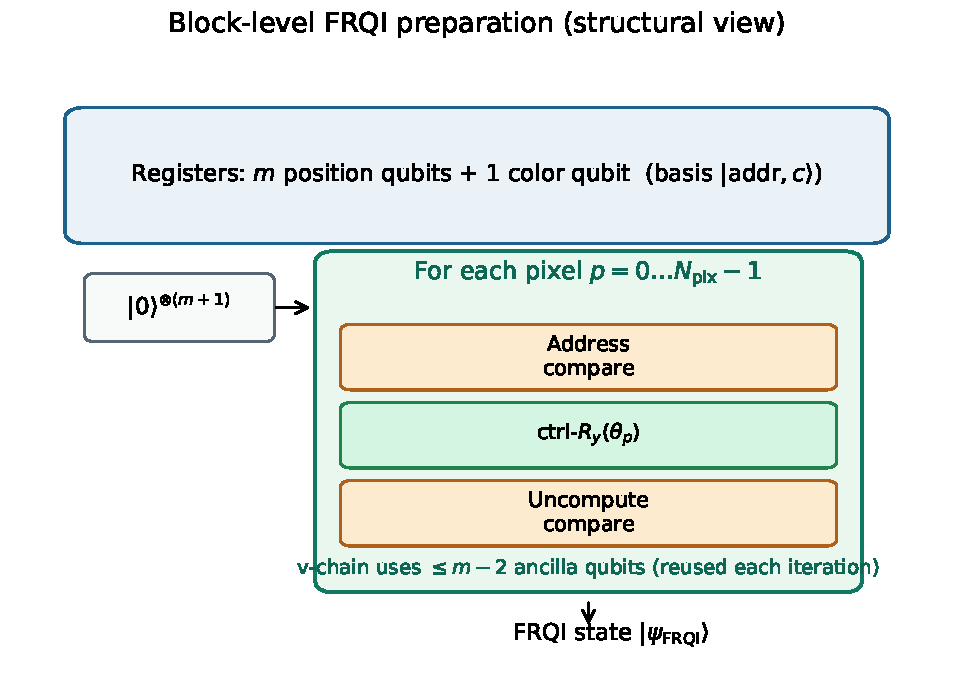
\includegraphics[width=0.92\textwidth]{block_frqi_prep.pdf}
\caption{Block-level view of the sequential FRQI preparation loop over pixels (registers, initialization, per-pixel compare--rotate--uncompute).}
\label{fig:block-frqi-prep}
\end{figure}

\subsection{End-to-end evaluation pipeline}
\Cref{fig:pipeline-flow} summarizes what the simulator exports to classical metrics: FRQI state preparation (structural variant), partial-trace decoding to an intensity raster, classical QHED post-processing, and scoring against the clean Sobel reference.

\begin{figure}[htbp]
\centering
\resizebox{\textwidth}{!}{%
\begin{tikzpicture}[
  font=\small,
  box/.style={rectangle, draw, rounded corners=2pt, align=center, inner sep=5pt, minimum width=2.2cm},
  arrow/.style={-{Stealth[length=2.2mm]}, thick},
]
\node[box, fill=blue!8] (enc) {FRQI preparation\\(naive or v-chain)};
\node[box, fill=blue!8, right=0.85cm of enc] (sim) {Aer simulator\\(DM / SV)};
\node[box, fill=green!10, right=0.85cm of sim] (dec) {Decode raster};
\node[box, fill=green!10, right=0.85cm of dec] (qhed) {QHED + Sobel ref};
\node[box, fill=orange!12, right=0.85cm of qhed] (score) {PSNR / SSIM /\\edge SSIM};
\draw[arrow] (enc) -- (sim);
\draw[arrow] (sim) -- (dec);
\draw[arrow] (dec) -- (qhed);
\draw[arrow] (qhed) -- (score);
\end{tikzpicture}%
}
\caption{Classical scoring path used in this thesis: identical QHED and references for naive and v-chain; only the preparation unitary (and its noise channel) changes. File-level mapping is summarized in the repository map table later in this chapter.}
\label{fig:pipeline-flow}
\end{figure}

\FloatBarrier

\subsection{Transpiled excerpt (Qiskit \texttt{MCXGate} v-chain)}
\Cref{fig:stub-mcx} shows a minimal Qiskit circuit diagram (saved from the repository stub helper) illustrating how a multi-controlled $X$ is expanded in v-chain mode before basis-gate transpilation---complementing the logical cartoons above.

\begin{figure}[H]
\centering
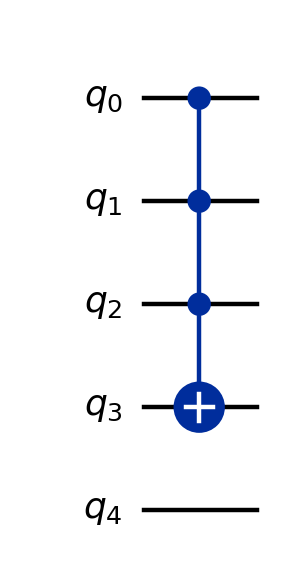
\includegraphics[width=0.55\textwidth]{stub_mcx_vchain.png}
\caption{Excerpt: \texttt{MCXGate} with \texttt{mode="v-chain"} on a few qubits (\texttt{outputs/stub\_mcx\_vchain.png}, from \texttt{scripts/qiskit\_stub\_draw.py}).}
\label{fig:stub-mcx}
\end{figure}

\section{Noise model}
Noisy simulations use Qiskit Aer with the \texttt{density\_matrix} method. Single-qubit depolarizing probability $p_1$ and two-qubit $p_2$ map a density matrix $\rho$ according to
\begin{equation}
\mathcal{E}_{\mathrm{1q}}(\rho) = (1-p_1)\rho + \frac{p_1}{3}\sum_{k\in\{X,Y,Z\}} P_k \rho P_k^\dagger ,
\end{equation}
and similarly for two-qubit channels on each CX site (implementation details in \texttt{src/noise\_models.py}). Thermal relaxation and readout hooks exist for API compatibility; unless a shot-based readout demo is enabled, readout noise does not alter the stored density matrix in the main noisy FRQI sweeps.

\begin{table}[htbp]
\centering
\caption{Synthetic noise grid used in the primary CSV bundle (each scale multiplies the baseline channel strengths).}
\label{tab:noise-grid}
\begin{tabular}{lrr}
\toprule
\texttt{noise\_scale} & $p_1$ (1q depolar) & $p_2$ (2q depolar) \\
\midrule
$0.0$ & $0$ & $0$ \\
$0.05$ & $0.0002$ & $0.001$ \\
$0.1$ & $0.0004$ & $0.002$ \\
$0.15$ & $0.0006$ & $0.003$ \\
$0.2$ & $0.0008$ & $0.004$ \\
\bottomrule
\end{tabular}
\end{table}

\section{Image and quantum metrics}
Let $\hat{I}$ be an $N\times N$ reconstruction and $I$ the ground-truth image. Mean squared error is $\mathrm{MSE}=\frac{1}{N_{\mathrm{pix}}}\sum_p (\hat{I}[p]-I[p])^2$. Peak SNR is
\begin{equation}
\mathrm{PSNR} = 10\log_{10}\frac{255^2}{\mathrm{MSE}} \quad (\mathrm{dB}) .
\end{equation}
SSIM is computed with scikit-image on \texttt{uint8} arrays (windowed, channel-wise for grayscale). State fidelity $F(\rho,\sigma)=\bigl(\mathrm{Tr}\sqrt{\sqrt{\rho}\sigma\sqrt{\rho}}\bigr)^2$ compares the simulated noisy state (partial trace to data register) to the ideal FRQI statevector.

\section{Readout mitigation (shot-based slice)}
Independently from depolarizing density-matrix runs, simulation of projective measurements takes place on the color qubit with a synthetic confusion matrix $A$, along with estimating outcome probabilities from finite shots, and applying a regularized inverse to obtain mitigated probabilities~\cite{Mu2025GuidedImageFiltering}. Details and notation follow \texttt{thesis/design/readout\_mitigation.md}; code entry point: \texttt{scripts/readout\_mitigation\_shot\_sweep.py}.

\section{Statistical comparisons}
For paired naive versus v-chain edge metrics it is reported exploratory Wilcoxon signed-rank tests on differences $\Delta = \mathrm{vchain}-\mathrm{naive}$ over the eight $(\mathrm{image},\mathrm{noise\_scale})$ pairs with $\mathrm{noise\_scale}>0$ in the primary CSV bundle. Readout mitigation is performed by pairing per-seed differences $\Delta_{\mathrm{seed}} = p_{1,\mathrm{mit}}-p_{1,\mathrm{raw}}$. These tests are \textbf{hypothesis-generating} only: multiplicity across metrics is not adjusted, and sample sizes are small.

\paragraph{Inclusion protocol.}
Rows enter the edge-metric pairing if and only if both \texttt{edge\_ssim\_naive} and \texttt{edge\_ssim\_vchain} are finite for the same tuple $(\mathrm{image},\mathrm{noise\_scale},\mathrm{topology},\mathrm{noise\_mode})$. At $16\times16$, v-chain columns are frequently \texttt{NaN} because density-matrix simulation is skipped; those cells are therefore excluded automatically, which reduces power but avoids imputing synthetic values. The Wilcoxon implementation is SciPy's two-sided test on paired differences; exact $p$-values are available because $n{=}8$ is small.

\paragraph{Interpretation guardrails.}
Even if $p<0.05$ is observed for a secondary metric such as fidelity, claims of ``statistically significant superiority of v-chain for edge quality'' are not made unless the edge-centric endpoints agree. Resource reductions and fidelity shifts can coexist with flat or negative edge SSIM because QHED couples nonlinearly to reconstruction noise and because the Sobel reference is not matched to QHED's spectral stage~\cite{Geng2022HybridNISQEdge}.

\section{Experimental setup}

\subsection{Simulator-only scope}
\textbf{All evidence remains simulator-only.} No IBM Quantum hardware shots are included, due to lack of hardware access; results use Qiskit Aer backends and synthetic noise grids.

\subsection{Data and software}
Datasets live under \texttt{data/test\_images/} as \texttt{test\_4x4.npy}, \texttt{test\_8x8.npy}, and \texttt{test\_16x16.npy}. The Python environment is pinned in \texttt{requirements.txt} (Qiskit~1.x, Qiskit Aer, NumPy, SciPy, pandas, Matplotlib, scikit-image). Three experiment tracks are executed: (1)~ideal FRQI+QHED baseline and \texttt{initialize} resource columns; (2)~structural resource CSVs and CX/depth plots; (3)~noisy reconstruction with optional readout mitigation slice.

\subsection{Transpilation settings}
Structural resource circuits are transpiled to basis gates \texttt{\{cx,rz,sx\}} at optimization level~3 with an unconstrained coupling map (resource study). The \textbf{frozen noisy FRQI and noisy-reconstruction bundles} referenced in \texttt{thesis/results\_configuration.md} instead pin \texttt{transpile\_optimization\_level=0} together with Qiskit~1.3.3 / Aer~0.16.4 and seed~42; this isolates noise sweeps from aggressive rewrite passes that could blur naive--v-chain comparisons. Readers should not mix CSV columns from different optimization levels without re-running both tracks at a common setting.

\subsection{Reproducible commands}
\begin{lstlisting}[language={}, basicstyle=\ttfamily\footnotesize, frame=single, breaklines=true]
# Ideal FRQI + QHED figures and encoding CSV
python scripts/frqi_qhed_sobel.py

# Structural resources (CSV + CX/depth plots)
python scripts/frqi_structural_resources.py

# Noisy FRQI sweep (16x16 v-chain optional via --allow-heavy-dm)
python scripts/noisy_frqi_sweep.py

# Noisy reconstruction -> QHED edge metrics (paired naive vs v-chain)
python scripts/noisy_recon_qhed_edge_metrics.py

# Readout mitigation multi-seed demo
python scripts/readout_mitigation_shot_sweep.py

# Regenerate thesis ingestion tables (requires PNGs if --require-figures)
python scripts/build_results_tables.py --require-figures
\end{lstlisting}

\subsection{Provenance}
Noisy and readout experiments are summarized in \texttt{thesis/results\_configuration.md}; JSON manifests in \texttt{outputs/experiment\_manifest\_*.json} record the Qiskit version, the random seed, and Git commit hashes when available.

Density-matrix simulation cost scales as $O(4^{n_q})$ in the worst case~\cite{NielsenChuang2010}; therefore $16\times16$ v-chain rows may be absent unless heavy-memory flags are enabled, and the Results chapter flags missing cells explicitly.

\FloatBarrier

\section{Repository map: modules and driver scripts}
\label{sec:repo-map}

\begin{table}[H]
\centering
\caption{Core modules and experiment drivers (selected).}
\label{tab:repo-map}
\small
\begin{tabular}{@{}p{4.2cm}p{4.8cm}p{4.6cm}@{}}
\toprule
\textbf{Concern} & \textbf{Module(s)} & \textbf{Script(s)} \\
\midrule
FRQI angles, address loop & \texttt{src/frqi.py} & \texttt{frqi\_qhed\_sobel.py} \\
Structural \texttt{MCXGate} modes & \texttt{src/improved.py} & \texttt{frqi\_structural\_resources.py} \\
QHED + Sobel scoring & \texttt{src/qhed.py} & \texttt{frqi\_qhed\_sobel.py}, \texttt{noisy\_recon\_qhed\_edge\_metrics.py} \\
Metrics (PSNR, SSIM, fidelity) & \texttt{src/metrics.py} & all image-quality paths \\
Depolarizing DM sweeps & \texttt{src/noise\_models.py} & \texttt{noisy\_frqi\_sweep.py} \\
Readout matrix inversion demo & (design in \path{thesis/design/}) & \texttt{readout\_mitigation\_shot\_sweep.py} \\
\bottomrule
\end{tabular}
\end{table}

\Cref{tab:repo-map} ties the mathematical objects in this chapter to Python modules and the scripts that produced the frozen CSV/PNG artifacts under \path{outputs/}. Structural transpiles use optimization level~3 (\path{frqi_structural_resources.py}); the noisy bundles in \path{thesis/results_configuration.md} use optimization level~0 for fair naive--v-chain comparisons.

\section{Computational workflow and software architecture}
Experiments are orchestrated as Python scripts that write CSV outputs and PNG figures under \texttt{outputs/}. The thesis ingestion script (\texttt{build\_results\_tables.py}) validates column contracts, compares CSV modification times to manifest timestamps, and emits Markdown and \LaTeX{} fragments under \texttt{thesis/generated/}. Committed excerpts under \texttt{thesis/bachelors\_en/generated/} keep the PDF buildable even when gitignored generated files are absent on a fresh clone.

\section{Design choices affecting comparability}
All noisy comparisons pair naive and v-chain rows from the same CSV export at identical tuples $(\mathrm{image},\mathrm{noise\_scale},\mathrm{topology},\ldots)$. When v-chain rows are missing, paired tests exclude those cells automatically. This is honest, but it reduces statistical power at $16\times16$. Transpilation uses a fixed optimization level so CX reductions reflect preparation structure rather than optimizer randomness.

\section{QHED post-processing steps (implementation view)}
Beyond the unitary FRQI core, the QHED reference path in \texttt{src/qhed.py} chains purely classical NumPy operations: (i)~extract an $N\times N$ intensity matrix from the simulator state; (ii)~apply a separable two-dimensional FWHT along rows and columns; (iii)~form a magnitude spectrum and invert the FWHT to return to the spatial domain; (iv)~convolve with the Sobel magnitude mask used for scoring. Step (iv) explains why the ``QHED versus Sobel'' SSIM is not identically one even in the noiseless limit: the quantum stage is not implementing classical Sobel directly~\cite{Yao2017QHED,QiskitTextbookQuantumEdgeDetection}.
